\documentclass{article}

\usepackage{url}
\usepackage{cite}
\usepackage[version=4]{mhchem}
\usepackage{graphicx}
\usepackage{subfigure}
\usepackage[a4paper,top=2cm,bottom=2cm,right=3cm,left=3cm,marginparwidth=1.75cm]{geometry}


\title{SARS-CoV-2 3CL Protease Gene Expression}
\author{Yan Haoming\\2300017744}
\date{September 13, 2024}

\begin{document}
\maketitle
\begin{abstract}
    In the last experiment, we had constructed recombinant plasmid vectors.
    Thanks for the help from teaching assistant, the plasmids had been sequenced and transferred from DH5$\alpha$ to BL21, the strain for gene expression.

    In this experiment, we enlarged the scale of bacterial growing by liquid culture until the cell population reached a given threshold measure by OD600.
    At that point we induced the gene expression by IPTG then analyzed the products by SDS-PAGE.
    However, the final result shown by SDS-PAGE did not follow our expectations.

    Apart from the detailed experimental methods as well as the basic principle behind them, I propose, in this report, three possible factors leading to unpredicted results which also should be the improvements in future experiment.
\end{abstract}
\textbf{Keywords: SARS-CoV-2, 3CL protease, liquid culture, OD600, IPTG, SDS-PAGE}
\section{Methods}
\subsection{Microbiological Culture: Liquid Culture}
In last week we had introduced recombinant DNA into \textbf{DH5$\alpha$} strain which were grown on \text{Agar Plate}.
With the help of teaching assistant, the DNA was then transferred to \textbf{BL21} strain which is able to express \textbf{T7 RNA polymerase} in the \textbf{Agar Plate.}
However, this week we want to grow up large amount of organism to produce protein, 
and therefore we need to culture the bacteria in \textbf{liquid medium}. Here is the detailed procedure.
\begin{itemize}
    \item Spread 4 mL liquid culture on the agar plate then divide into 3 groups equally.
    \item Transfer the liquid containing bacteria back to the \textbf{Erlenmeyer Flask (Conical Flask)} with the volume of 1,600 $\mu$L per flask.
    \item Add 150 $\mu$L \textbf{ampicillin} to each of flask(150 mL) with the ratio of 1 : 1000 to construct a selective medium. 
    The 3 groups were designated 3CL1, 3CL2 and 3CL3 respectively.
    \item Store the cultures inside the \textbf{incubator} at 37 $^\circ$C.
\end{itemize} 
The incubator containing the liquid culture is shown in Figure \ref{Incubation}

\begin{figure}
    \centering
    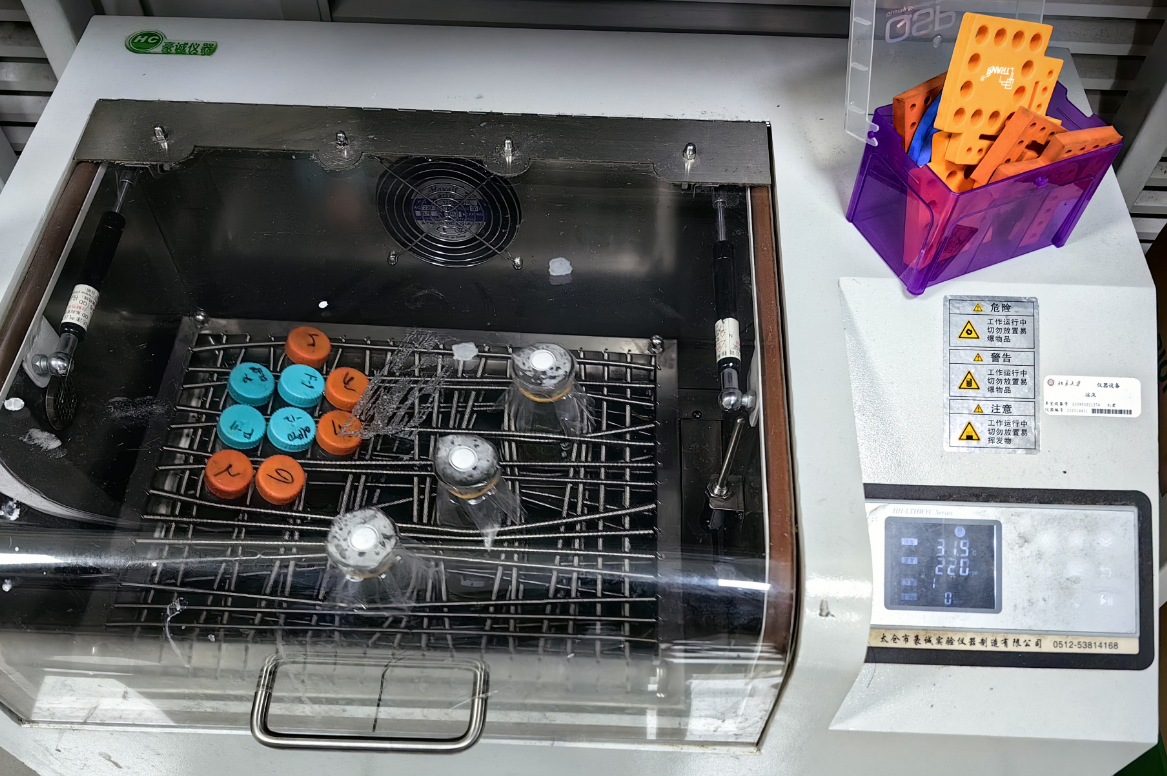
\includegraphics[width=0.5\linewidth]{../Figures/Incubation.png}
    \caption{Incubation}
    \label{Incubation}
\end{figure}
\subsection{Estimating Bacterial Concentrations: OD600 Spectrometry}
To determine the stage of growth of the bacterial cells, we harnessed the spectrometer to detect the value of \textbf{optical density at wavelength of 600 nm (OD600)}. 
We had been waiting 2 hours before measuring OD600 since putting into incubator. We sampled the bacteria (2 $\mu$L) for test every 20 minutes until the value of OD600 reached 0.8. 
The final results are shown in Figure \ref{OD600 Value Detection}.
Once the OD600 value exceeded 0.8, we cooled it above ice to repress further proliferating.

\begin{figure}
    \centering
    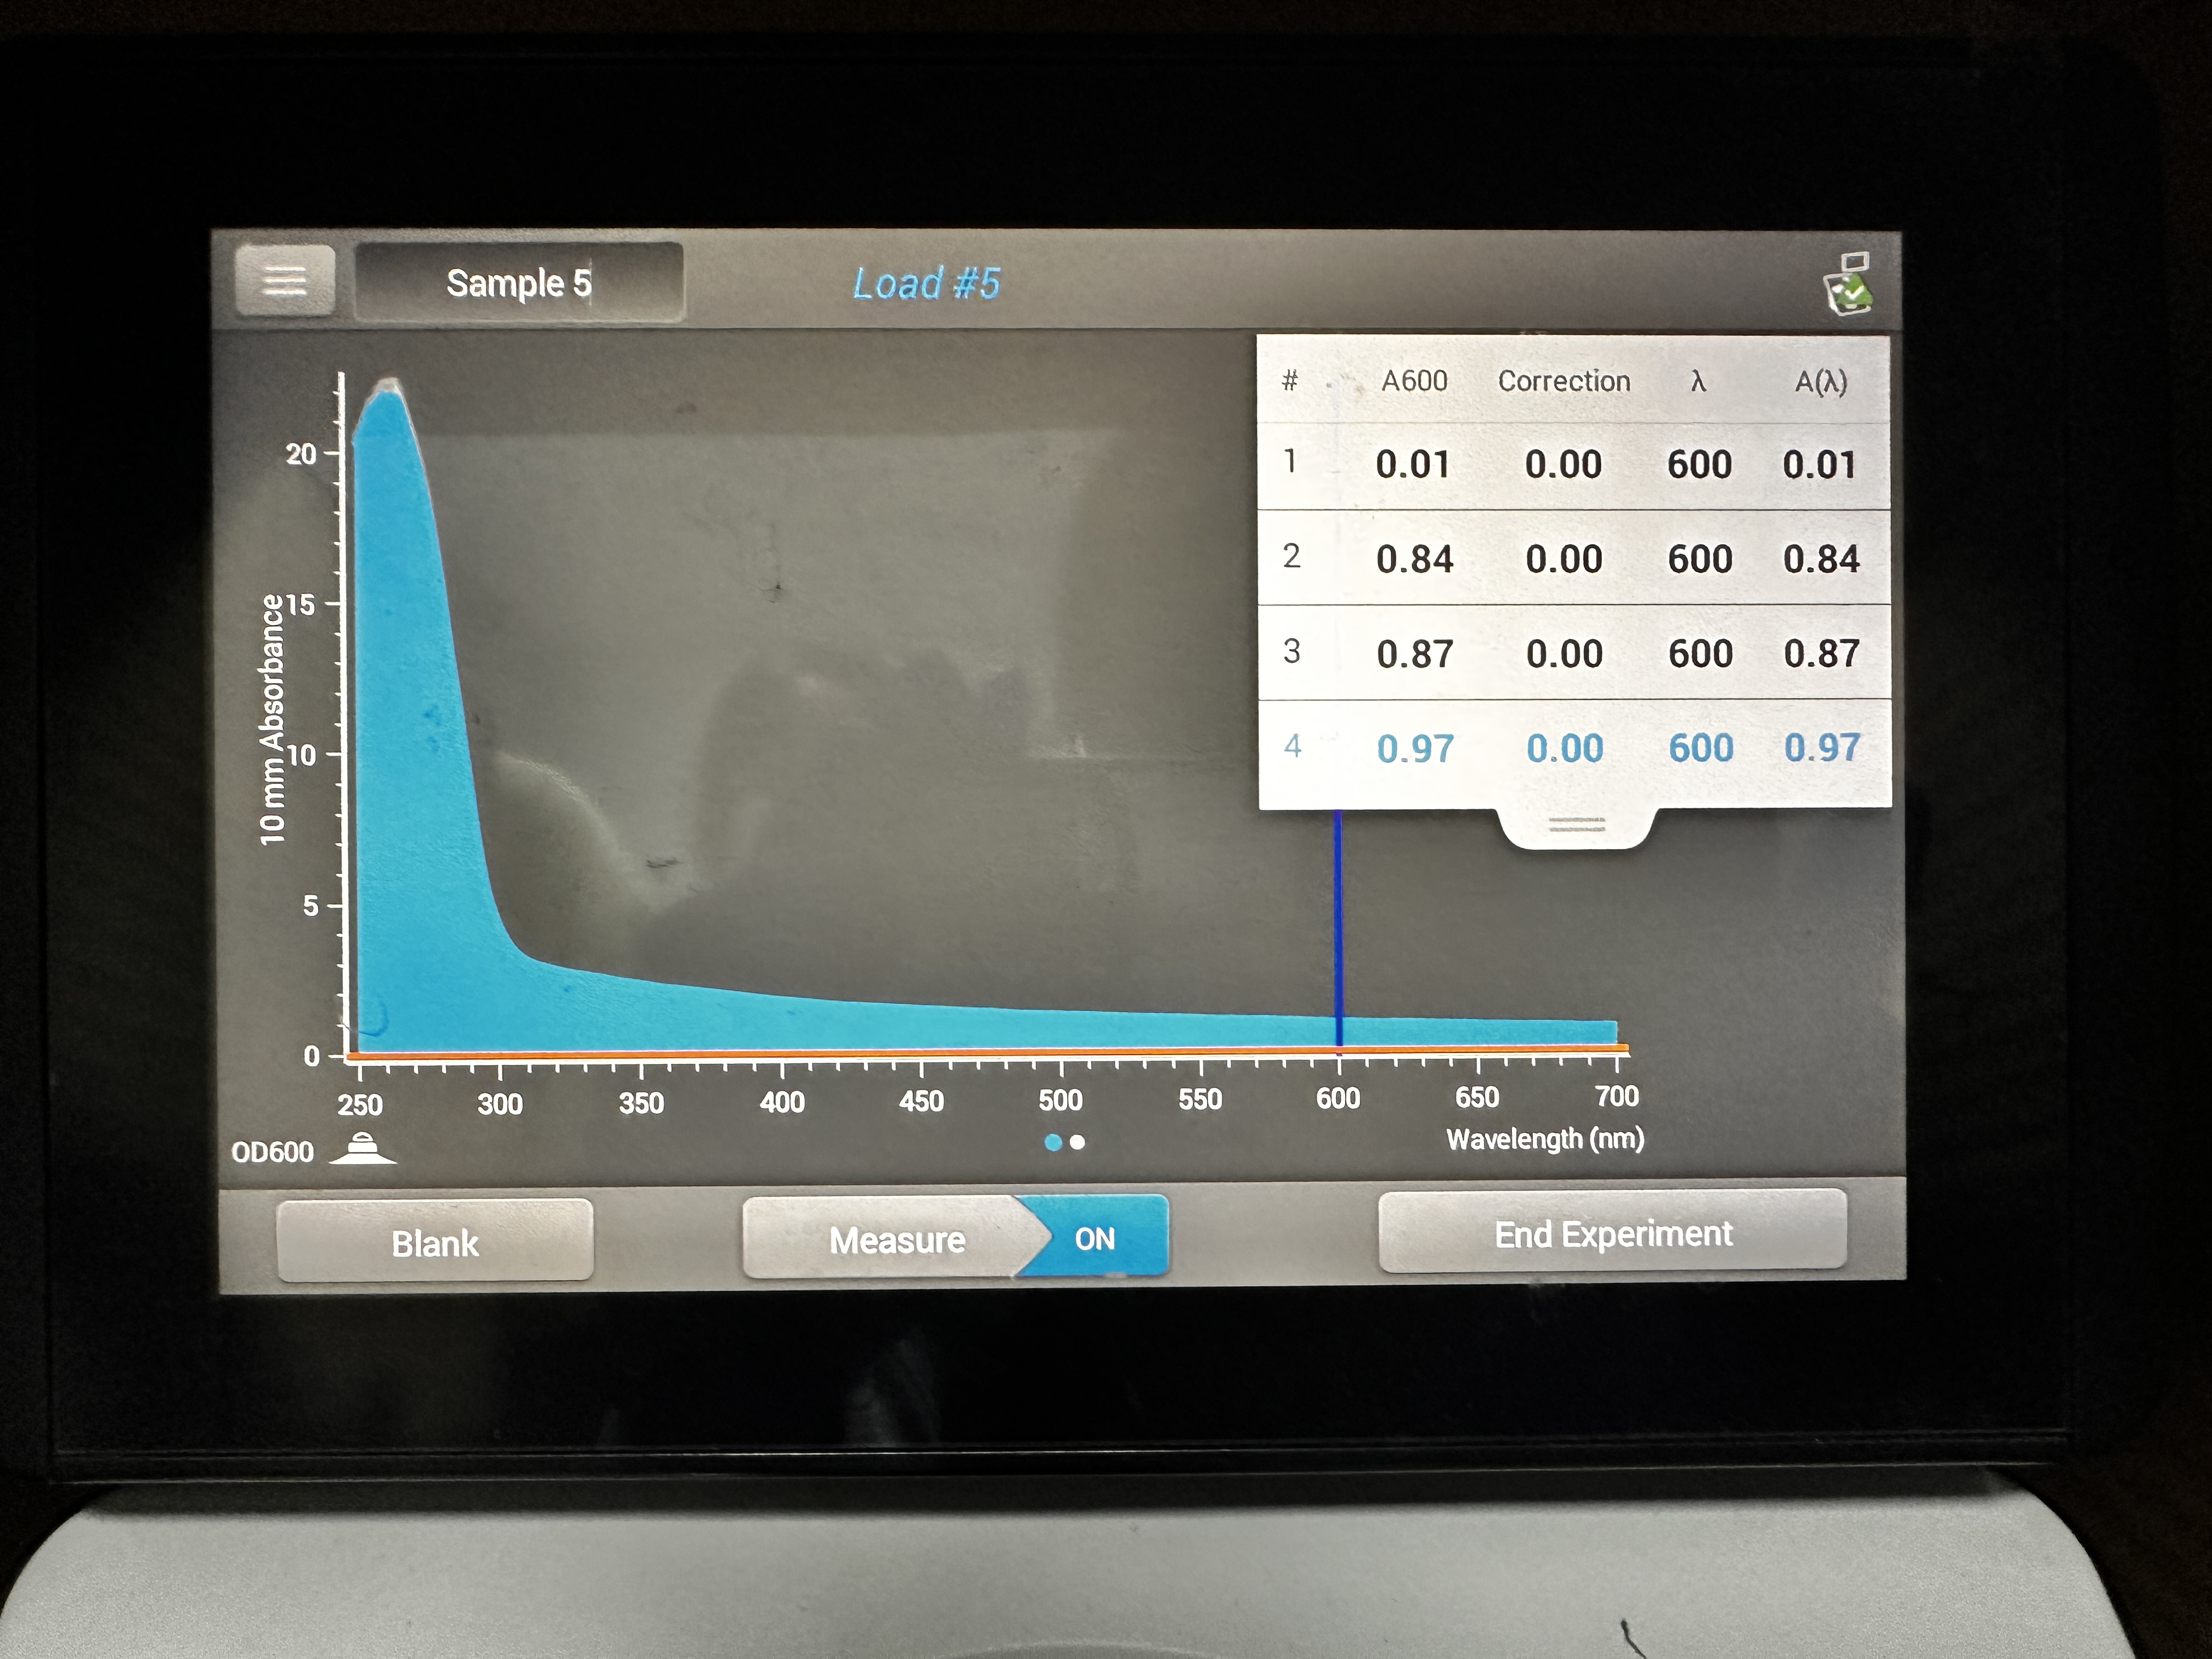
\includegraphics[width=0.7\linewidth]{../Figures/OD600.jpg}
    \caption{OD600 Value Detection}
    \label{OD600 Value Detection}
\end{figure}

\subsection{Induce Gene Transcription: IPTG}
The expression vector has \textit{Lac operator} as \textit{cis}-regulatory sequence and \textit{LacI} to express \textit{Lac inhibitor} which binding to \textit{Lac operator} to repress the transcription of 3CL protease gene.
To relieve that repression we added IPTG which is an analogue of allolactose aimed at inducing the expression of 3CL protease gene. 
The ratio was also 1 : 1000, which meant 150 $\mu$L IPTG per flask (150 mL).
\subsection{Protein Separation and Analyzing: SDS-PAGE}
We separated and analyzed the protein by \textbf{Sodium Dodecyl Sulfate-Polyacrylamide Gel Electrophoresis.} 
\subsubsection{Gel Preparation}
The gel sandwiched between 2 glass plates can be divided into 2 parts: \textbf{stacking gel and separating gel}. We prepared them respectively with slightly different constituents.

As for the separating gel (10 mL), the following ingredients were used:
\begin{itemize}
    \item 4.6 mL \ce{ddH2O}
    \item 2.7 ml 30\% acrylamide
    \item 2.5 mL \textbf{1.5M Tris-HCl (pH 8.8)}
    \item 0.1 mL 10\% SDS
    \item 0.1 mL 10\% \ce{(NH4)2S2O8}
    \item 6 $\mu$L TEMED (Tetramethylethylenediamine)
\end{itemize} 

As for the stacking gel (4 mL), the following ingredients were used:
\begin{itemize}
    \item 2.7 mL \ce{ddH2O}
    \item 0.67 ml 30\% acrylamide
    \item 0.5 mL \textbf{0.5M Tris-HCl (pH 6.8)}
    \item 0.04 mL 10\% SDS
    \item 0.04 mL 10\% \ce{(NH4)2S2O8}
    \item 4 $\mu$L TEMED (Tetramethylethylenediamine)
\end{itemize}
The major difference lies in the pH caused by the concentration of buffer.
\subsubsection{Sample Preparation}
Before loading the sample, we added loading buffer (20 $\mu$L) to the bacteria (50 $\mu$L) heating at 98$^\circ$ for 20 minutes.
Then centrifuged for 5 minutes at the speed of 12,000 rmp.
The desired protein should dissolve in the supernatant and therefore we kept the supernatant abandoning the pellet.
\subsubsection{Electrophoresis}
We loaded 10 $\mu$L sample per lane with 4 $\mu$L marker (protein ladder).
The electrophoresis apparatus is shown in Figure \ref{OD600 Value Detection}
\begin{figure}
    \centering
    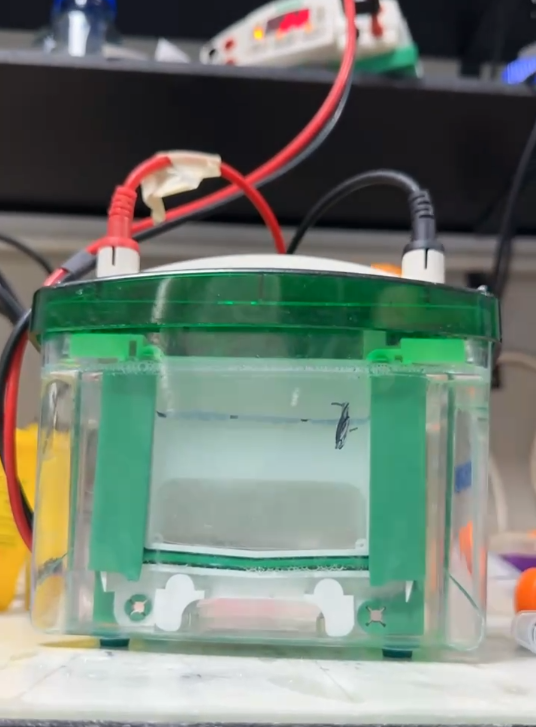
\includegraphics[width=0.5\linewidth]{../Figures/SDS-PAGE.png}
    \caption{SDS-PAGE}
    \label{SDS-PAGE}
\end{figure}
\subsubsection{Staining}
To take photograph of the separated gel, we stained the gel by \textbf{Coomassie Brilliant Blue} heating within the microwave oven for a short period.
Since the Coomassie brilliant blue stained the polyacrylamide gel altogether, we should destain the gel in solution to highlight the stained protein.
The gel was soaked in destaining solution exchanging the solution every 2 hours.
The result is shown in Figure \ref{SDS-PAGE Result}.
\begin{figure}
    \centering
    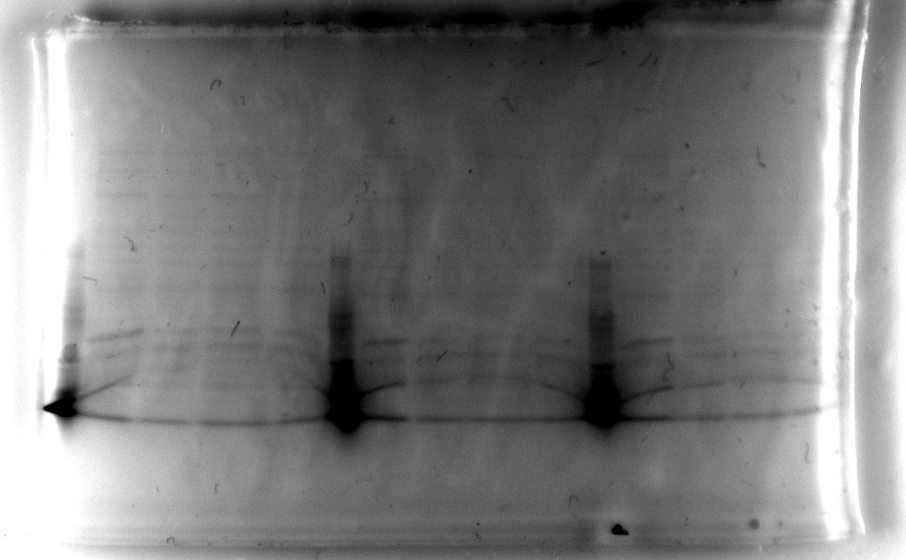
\includegraphics[width=0.7\linewidth]{../Figures/SDS-PAGE Photograph.png}
    \caption{SDS-PAGE Result}
    \label{SDS-PAGE Result}
\end{figure}
\section{Experimental Results}
It is a pity that we do not get predicted results after SDS-PAGE according to Figure \ref{SDS-PAGE Result}.
And there can be several possible causes for that.

First of all, the marker (protein ladder) did not mark the molecular wright exactly and obviously, which meant the deficiency in marker.
Maybe testing of marker before electrophoresis will enable better resolution in SDS-PAGE photograph.

Although we can not tell the obvious difference between the lane of controlled group (not induced by IPTG) and the other 2 groups, successful inducing of gene expression (in major experiment and have not been analyzed) can not be ruled out.
Given the limitation of time, the protein used for SDS-PAGE had been prepared in preliminary experiment with a smaller scale.
Besides, the loading amount may be insufficient for the purpose of clear observations, which means even the gene was successfully expressed, we would still miss it.
According to the above reasoning, inadequate loading amount and small scale in the preliminary experiment might be the factor causing unpredicted results.

To support this idea, I want to cite a photograph \cite{TheCell} in Figure \ref{Proteins Present at Successive Stages in the Purification} where the band is broad enough and thus be obvious to see only when it is purified and account for a large proportion in the sample.
\begin{figure}
    \centering
    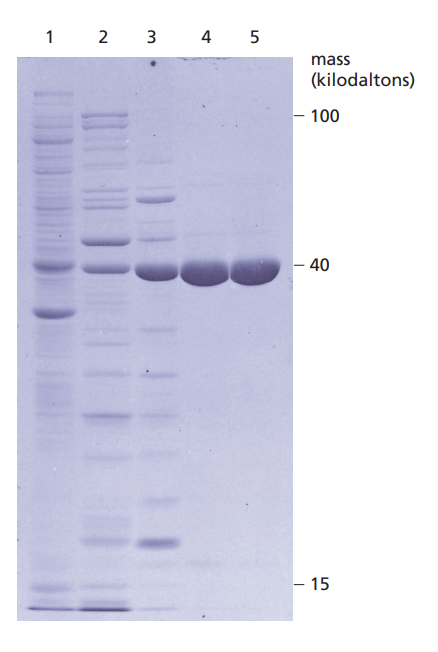
\includegraphics[width=0.3\linewidth]{../Figures/SDS-PAGE from the cell.png}
    \caption{Proteins Present at Successive Stages in the Purification \cite{TheCell}}
    \label{Proteins Present at Successive Stages in the Purification}
\end{figure}

Next time, both the checking of marker (protein ladder) and appropriate loading amount as well as bacterial culture scale should the major improvements.



\bibliographystyle{plain}
\bibliography{references}
\end{document}